\documentclass{standalone}
\usepackage{tikz}
\begin{document}
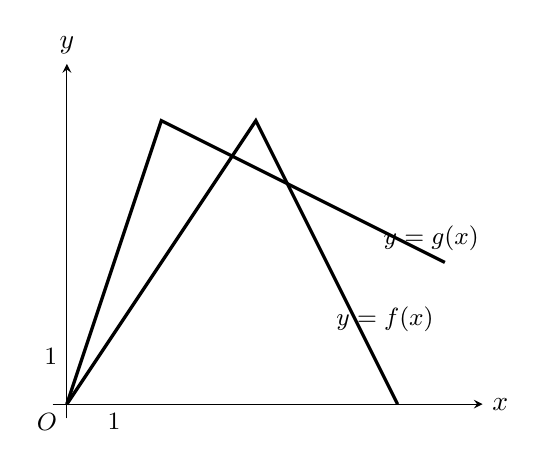
\begin{tikzpicture}[>=stealth, scale=0.6]
  % Axes
  \draw[->] (-0.3,0) -- (8.8,0) node[right] {$x$};
  \draw[->] (0,-0.3) -- (0,7.2) node[above] {$y$};

  \begin{scope}
    \clip (-0.3,-0.3) rectangle (8.8,7.1);
    % g(x): (0,0)->(2,6) slope 3, then (2,6)->(8,3) slope -1/2
    % g(6)=4, g'(6)=-1/2  [verified: 6 - (1/2)(6-2)=4]
    \draw[very thick] (0,0) -- (2,6) -- (8,3);
    % f(x): (0,0)->(4,6) slope 3/2, then (4,6)->(7,0) slope -2
    % f(6)=2, f'(6)=-2  [verified: 6 - 2(6-4)=2]
    \draw[very thick] (0,0) -- (4,6) -- (7,0);
  \end{scope}

  % Function labels (placed where g is clearly above f)
  \node[right,font=\small] at (6.5,3.5) {$y = g(x)$};
  \node[right,font=\small] at (5.5,1.8) {$y = f(x)$};

  % Axis labels
  \node[below left,font=\small] at (0,0) {$O$};
  \node[below,font=\small] at (1,0) {$1$};
  \node[left,font=\small]  at (0,1) {$1$};
\end{tikzpicture}
\end{document}
